\section{\scAssesmentHeader{Финляндии}}


% \subsection{\scAssesmentBuildingClass}
% % 
% \subsection{\scAssesmentBuildingMetrics}

% ##########-----Регулирование


\subsection{\scAssesmentBuildingLaw}
% 
Политика на уровне государства направлена на обеспечение мер по преодолению грядущего глобального энергетического кризиса,
государство видит национальную безопасность основой бесперебойных поставок энергии и, в свою очередь, энергию ---
как основу общества и его развития для будущего \cite{law_FIN_govMinEnvSecurity}. Эта позиция находит отражение как основополагающее направление в домостроении.

Большинство финнов живут в частных домах. Одним из основных преимуществ жилья, занимаемого владельцем, по сравнению с арендованным жильем является то,
что часть расходов на жилье, например, взносы по ипотеке, может учитываться как сбережения.

Ministry of the Environment\footnote{рус. Министерство окружающей среды} ведает полномочиями и правовыми актами,
регулирующими взаимодействие человека и жилой среды. Цель министерства окружающей среды заключается в обеспечении адекватного предложения различных видов жилья на рынке жилья,
направлении строительной отрасли и жилищного строительства в направлении, которое является экологически устойчивым, и расширении возможностей жителей влиять на свои жилищные условия.
В министерстве окружающей среды ответственность за жилищное строительство возложена на Департамент антропогенной среды.
Субсидии, субсидии и гарантии, связанные с жильем и строительством, предоставляются Центром финансирования и развития жилищного строительства Финляндии (АРА),
который также руководит и контролирует использование субсидируемого государством строительного фонда АРА.

На уровне субъекта (региональном) действует Regional plan and land use planning, регламентируемый The Land Use and Building Act 132/1999 28 §\footnote{рус. Закон о землепользовании и строительстве},
устанавливющий требования к содержанию регионального плана \cite{law_FIN_RulesCode_LanduseAndBuilding}.
Региональное планирование включает в себя: региональную схему, региональный план, программу регионального развития.
Региональный план представляет собой карту, подготовленную в соответствии с Законом о землепользовании и строительстве, отображающую планы землепользования и структуры общин региона.
В нем описывается строительство и экологическое развитие в ближайшие десятилетия. Региональный план содержит инструкции по муниципальному планированию землепользования и другим официальным мероприятиям, которые влияют на землепользование.
Региональные планы составляются и утверждаются областными советами.
Несколько факторов влияют на муниципальную политику землепользования (планы землепользования и земельная политика).
К ним относятся фактические процессы планирования землепользования и другие виды планирования землепользования, а также промышленная, социальная и жилищная политика.
К числу инструментов планирования землепользования муниципалитетов относятся следующие:
\begin{itemize}
    \item стратегии и программы землепользования в муниципалитете;
    \item местный генеральный план и местный план территории;
    \item земельная политика;
    \item постановление о строительстве.
\end{itemize}
Региональный план определяет, как земля используется в регионе. Местный генеральный план устанавливает цели землепользования в муниципалитете.
В нем излагается общее развитие муниципалитета и использование земельной площади, которую он охватывает, например, расположение жилых районов, мест работы и транспортных маршрутов.
Можно подготовить частичный генеральный план для таких районов, как берега. Такой план может быть более подробным, чем местный генеральный план.
Каждый муниципалитет несет ответственность за подготовку местного генерального плана.
Этот план утверждается муниципальным советом. Если муниципалитеты подготовят общий местный генеральный план, он будет утвержден общим органом муниципалитетов и утвержден министерством окружающей среды.
Закон о землепользовании и строительстве устанавливает требования к содержанию местного генерального плана.
Местный генеральный план используется в качестве основы для подготовки местных подробных планов.


Сбор обратной связи от интересантов территории в ходе разработки документов на всех уровнях принятия решений осуществляется средствами государственных информационных систем
и георафических порталов. В настоящее время в финском государственном управлении проводятся широкомасштабные реформы, направленные на совершенствование управления информацией
и ее использования. Благодаря этим реформам информация, содержащаяся в различных регистрах центральных и местных органов власти, будет соответствовать международным стандартам и
будет более функционально совместимой и пригодной для использования, чем раньше. За информацию о антропогенной среде отвечает главным образом министерство окружающей среды.
Цифровизация административного сектора осуществляется в министерстве в рамках двух широких образований.
Цель состоит в том, чтобы создать основу для общенациональных электронных услуг в сфере недвижимости и строительства, а также для новых возможностей для бизнеса.
Другим аспектом работы в области развития является функциональная совместимость информации о антропогенной среде, поощряемая широкой группой по сотрудничеству.
Вторым объектом является четырехлетний проект Ryhti, который готовит общенациональную информационную систему для антропогенной среды.
Эта работа изложена в Законе о землепользовании и строительстве, который в настоящее время пересматривается.
В его основные задачи входит повышение качества строительства и содействие цифровизации.


Таким образом, регулирование вопросов энергоэффективности зданий Финляндии органично включено в структуру законодательства и реализуется как системный подход,
связанный с территориальным планированием и управлением развитием территориями. Технологии информационного моделирования тесно интегрируются с сообществом и застройщиками,
позволяя реализовать комплексные подходы к оценке и оптимизации параметров энергопотребления зданий при застройке.

% ##########-----Опыт


\subsection{\scAssesmentExp}

Большинство финнов живут в частных домах. Одним из основных преимуществ жилья, занимаемого владельцем, по сравнению с арендованным жильем является то,
что часть расходов на жилье, например, взносы по ипотеке, может учитываться как сбережения. Однако покупка дома обычно влечет за собой получение кредита,
что делает его существенным и долгосрочным. срочное экономическое обязательство, требующее тщательного рассмотрения.
% \clearpage
\begin{figure}
    \centering
    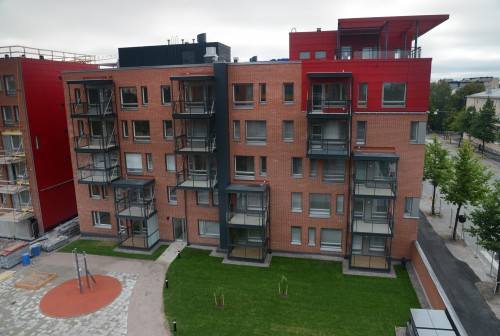
\includegraphics[width=\textwidth]{assets/figures/st1ch03_finexp_001.png}
    \caption{Социальное крупнопанельное жильё в Финляндии (фотоснимок из ресурса https://iti-consulting.ru/dostupnoe-zhile-finskij-opyt-foto/)}
    \label{fig:st1ch03_finexp_001}
  \end{figure}


В крупных населённых пунктах Арктики, таких как Оулу, преобладает микрорайнная застройка блокированными секциями в виде линейных и перемитральных фронтов застройки,
реализуемая с целью компактного распределения инженерных сетей и энергосбережения посредством предотвращения потерь тепла.
Эти объекты возводятся с применением железобетонных каркасов и крупнопанельных модулей (Рисунок \ref{fig:st1ch03_finexp_001}).

